\documentclass[mathserif]{intbeamer}
%\usepackage{etex}
\usepackage[utf8]{inputenc}
\usepackage[english]{babel}
%\usepackage{qrcode}
%\usepackage[space]{grffile}
\usepackage{subcaption}
\captionsetup[subfigure]{skip=-5pt} % global setting for subfigure
%\usepackage{aligned-overset}
\usepackage{amsmath,amssymb,amsfonts}
\usepackage{trfsigns}
\usepackage{gensymb}

\usepackage{../paper/macros}
\usepackage{xcolor}
\usepackage{enumerate}

\makeatletter
\def\mathcolor#1#{\@mathcolor{#1}}
\def\@mathcolor#1#2#3{%
  \protect\leavevmode
  \begingroup
    \color#1{#2}#3%
  \endgroup
}
\makeatother


%% *** Tikz, PGF and AudioIcons ***
%\usepackage{tikz, audioicons}
%\usetikzlibrary{calc,%
%  decorations.pathreplacing,%
  % decorations.markings,%
  % calc,%
  % arrows,%
  % through,%
  % intersections,%
  % positioning}

%\definecolor{activecolor}{RGB}{255, 0, 0}
% \definecolor{loudspeakercircle}{RGB}{236, 236, 236}
% \definecolor{focuscircle}{RGB}{254, 204, 0}
% \definecolor{darkgreen}{rgb}{0,0.5,0}
% \definecolor{orange}{rgb}{1.0,0.5,0}
% \definecolor{mauve}{RGB}{224,176,255}
% \definecolor{teal}{RGB}{64,224,208}

% \makeatletter
% \tikzset{
%   dot diameter/.store in=\dot@diameter,
%   dot diameter=3pt,
%   dot spacing/.store in=\dot@spacing,
%   dot spacing=10pt,
%   dots/.style={
%     line width=\dot@diameter,
%     line cap=round,
%     dash pattern=on 0pt off \dot@spacing
%   }
% }
% \makeatother

%% *** Importing Stuff ***
%\usepackage{import}

%% *** Mathsymbols ***
%\usepackage{soundfield}
%\sfrenewsymbol{cylm}{\mu}

%\usepackage{nicefrac}
%\DeclareFontFamily{U}{wncy}{}
%\DeclareFontShape{U}{wncy}{m}{n}{<->wncyr10}{}
%\DeclareSymbolFont{mcy}{U}{wncy}{m}{n}
%\DeclareMathSymbol{\Sha}{\mathord}{mcy}{"58}

%% *** Additional Commands extending Beamer ***
%\newcommand{\itemplus}[1][+]{\item[\textcolor{darkgreen}{\textbf{#1}}]}
%\newcommand{\itemminus}[1][--]{\item[\textcolor{red}{\textbf{#1}}]}
%\newcommand{\itemattent}[1][!\,]{\item[\textcolor{orange}{\textbf{#1}}]}
%\newcommand{\itemcheck}{\itemplus[$\checkmark$]}
%\newcommand{\itemcross}{\itemminus[$\boldsymbol{\times}$]}

%\newenvironment{itemizeblock}[1]{ %
%  \begin{block}{#1} %
%    \begin{itemize} %
%    } %
%    { %
%    \end{itemize} %
%  \end{block} %
%} %

\setbeamercovered{invisible}

% ===== titlepage info =====
\title[Audibility Constant Phase Shifts]%
  {Detection of Constant Phase Shifts in\\Filters for Sound Field Synthesis}

\author[Schultz, Hahn, Spors]{%
    \underline{Frank Schultz},
    Nara Hahn,
    Sascha Spors
}

\date[2019-09-28]{%
  5th ICSA, Ilmenau, ORAL-5-3\\
}

\institute[]{Institute of Communications Engineering, University of Rostock}

% ===== remove total number of slides from pagenumber =====
\setbeamertemplate{page number in head/foot}[nototal]
\setbeamersize{text margin left=\logomargin}
\setbeamertemplate{blocks}[rounded]
\setbeamercolor{block title}{fg=rostock-uni, bg=white}

\begin{document}
\maketitle
%
%
%
\section{Introduction}
\begin{frame}{Sound Field Synthesis (SFS) with Linear / Planar Arrays}
\begin{columns}[T]
\column{0.33\textwidth}
2.5-dimensional SFS

\hspace{1cm}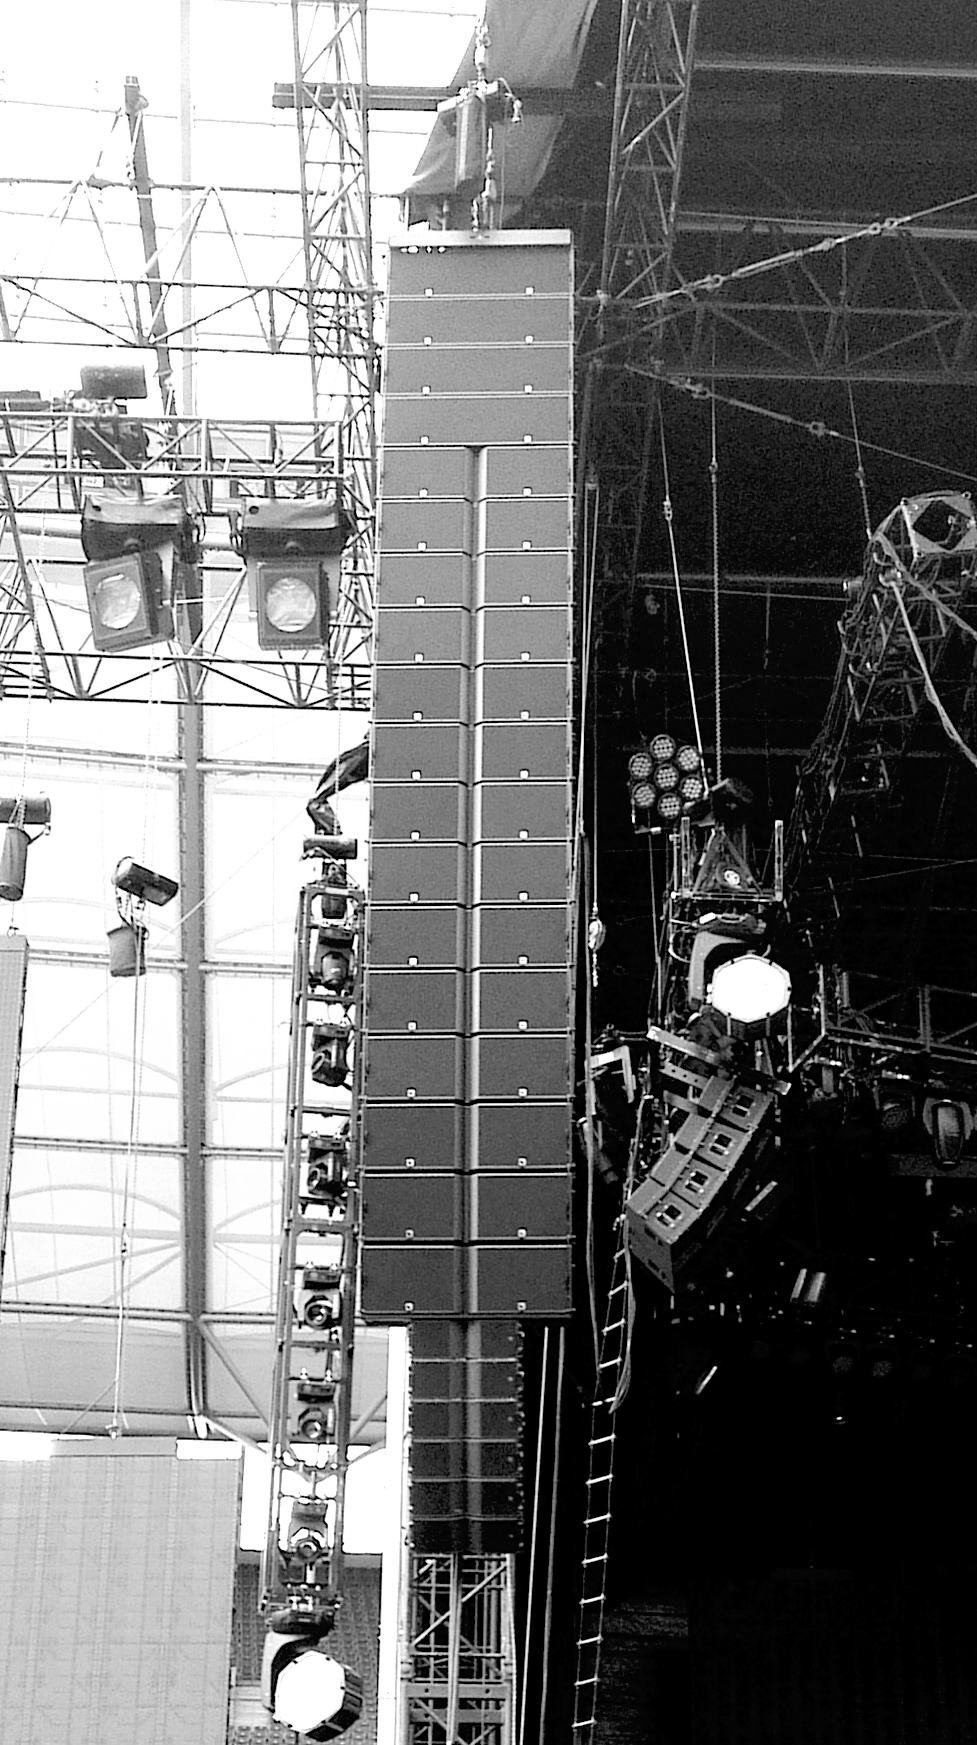
\includegraphics[width=0.5\textwidth]{graphics/lineararray}
\column{0.67\textwidth}
\only<1>{
ideal half-derivative EQ for infinite linear array

\includegraphics[width=1\textwidth]{graphics/equalizer-ideal-line-source}
}
\only<2>{
ideal half-derivative EQ for infinite linear array

\includegraphics[width=1\textwidth]{graphics/equalizer-ideal-line-source}
}
\only<3>{
ideal half-derivative EQ for infinite linear array

\includegraphics[width=1\textwidth]{graphics/equalizer-ideal-line-source}
}
\end{columns}
\vspace{0.25cm}
\begin{columns}[T]
\column{0.33\textwidth}
\only<1>
{
3-dimensional SFS

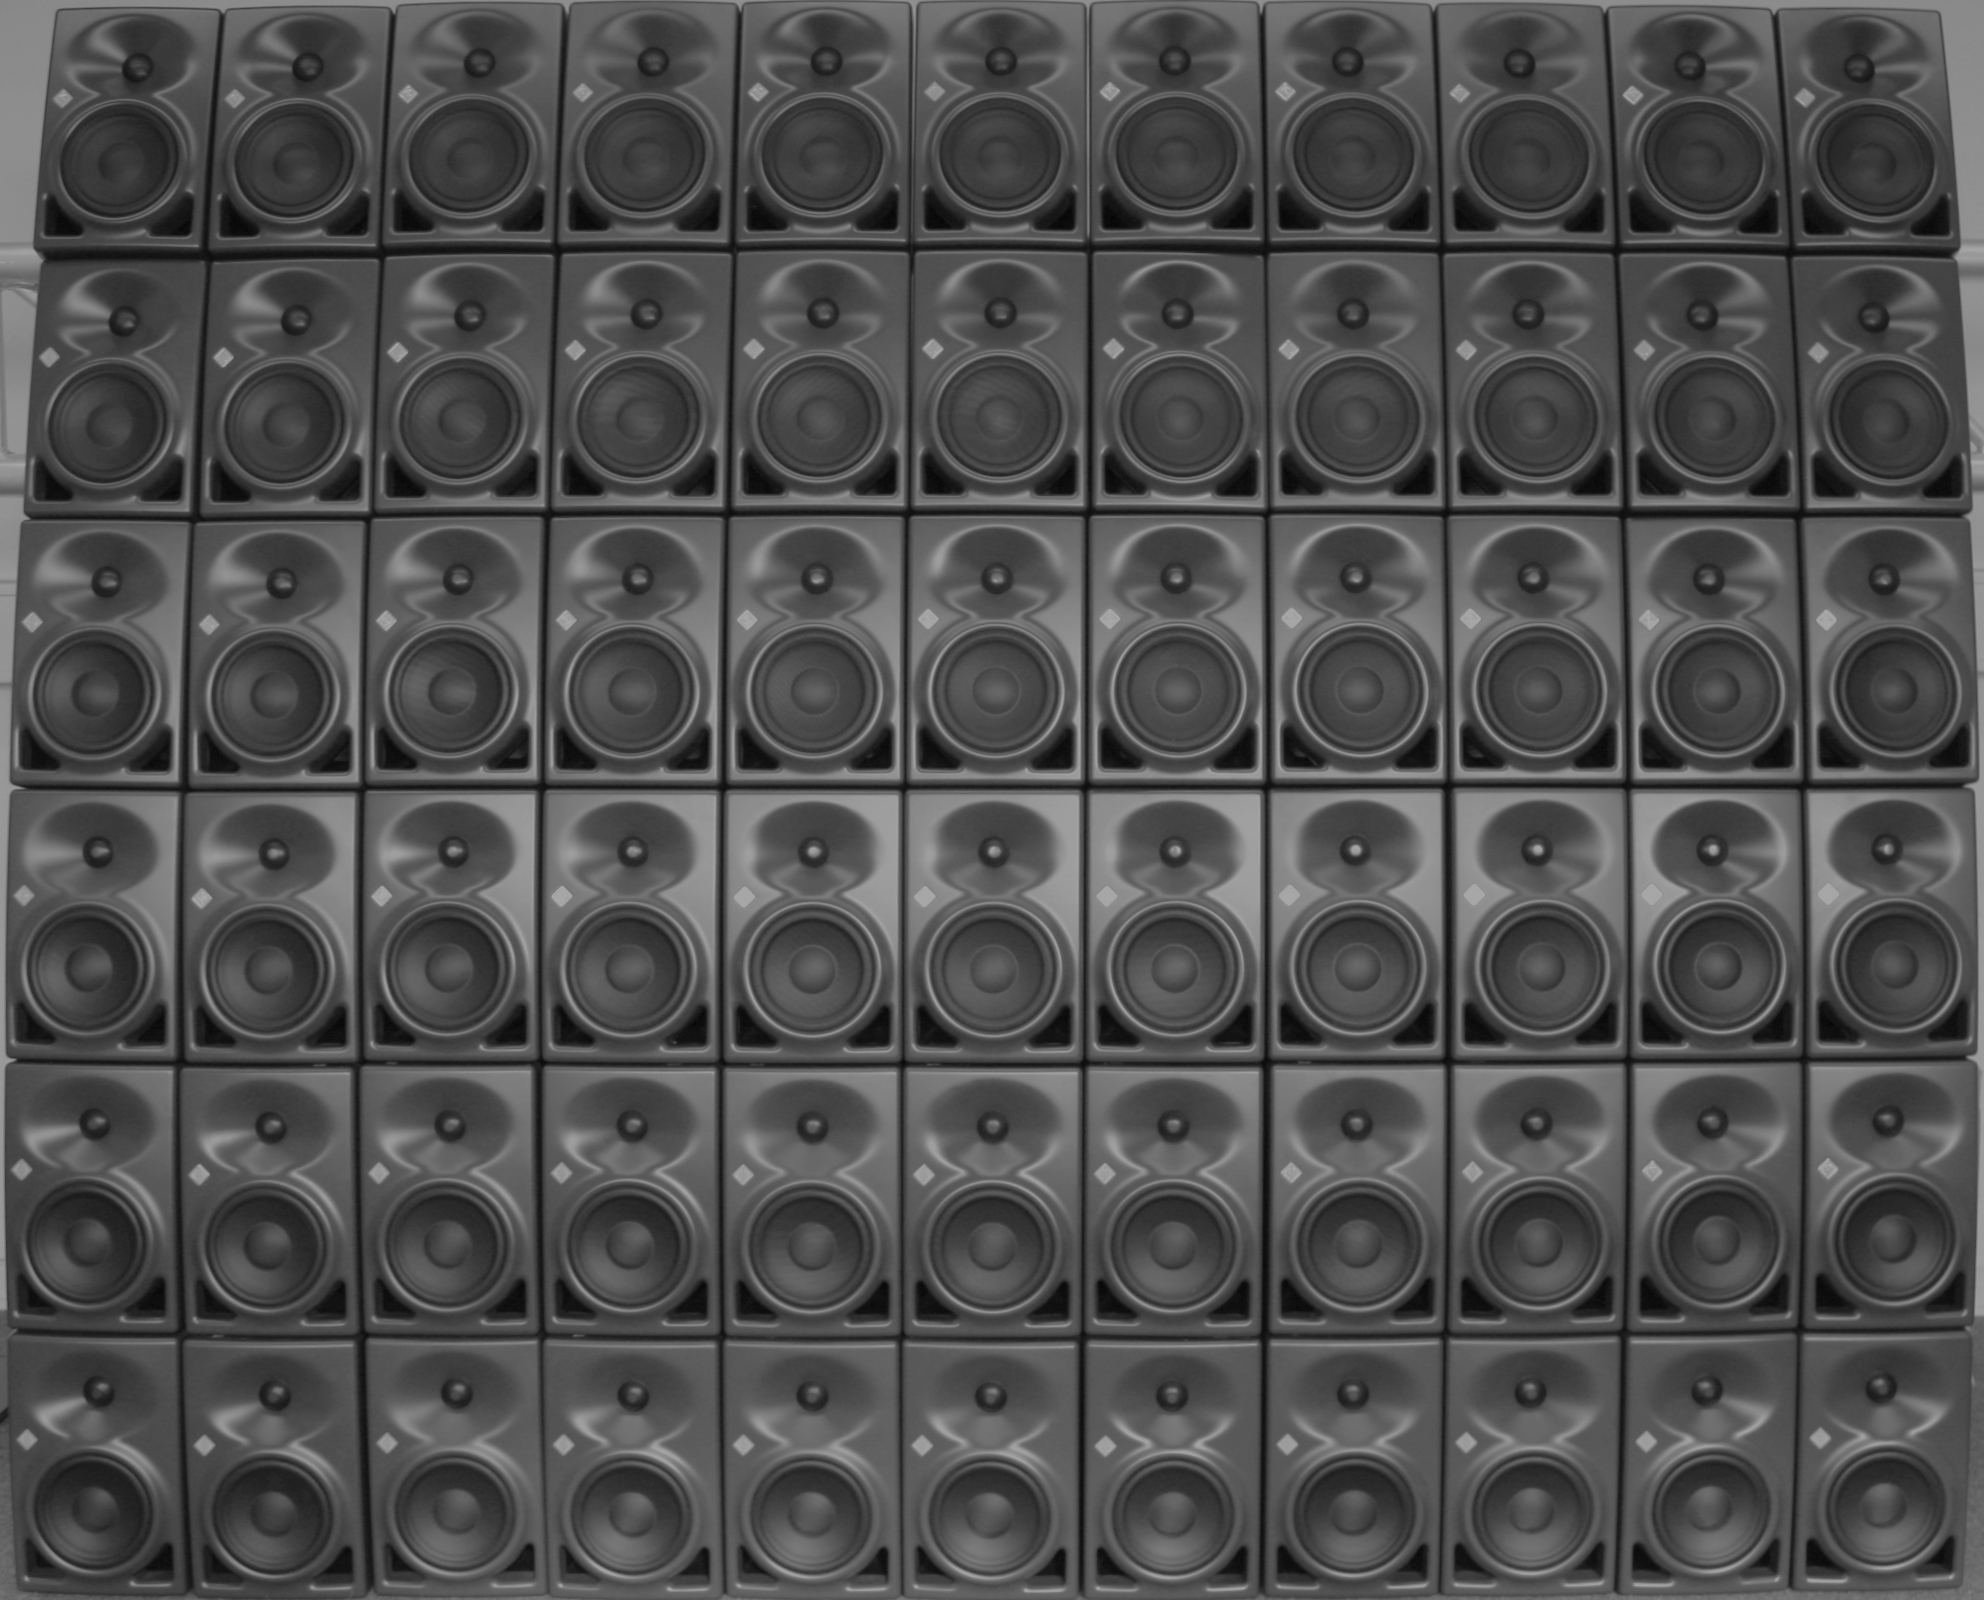
\includegraphics[width=1\textwidth]{graphics/planararray}
}
\column{0.67\textwidth}
\only<1>{
ideal full-derivative EQ for infinite planar array

\includegraphics[width=1\textwidth]{graphics/equalizer-ideal-plane-source}
}
\only<2>{
half-derivative slope for finite length array, minimum phase

\includegraphics[width=1\textwidth]{graphics/equalizer-minimum-phase}
}
\only<3>{
half-derivative slope for finite length array, linear phase

\includegraphics[width=1\textwidth]{graphics/equalizer-linear-phase}
}
\end{columns}
\end{frame}
%
%
%
\begin{frame}{Ideal Constant Phase Shift}
\begin{figure}
\includegraphics[width=0.8\textwidth]{graphics/ideal-spectra-and-square-waves}
\end{figure}
\end{frame}
%
%
%
\begin{frame}{Literature}
\textbf{Audio Engineering Context}:
\small

[13] V. Hansen E. R. Madsen (1974): "On aural phase detection" \textit{JAES}
22(1)%:10–14

[14] --- (1974): "On aural phase detection: Part II" \textit{JAES}
22(10)%:783–788

[15] J. Blauert, P. Laws (1978): "Group delay distortions in electroacoustical
systems" \textit{JASA} 63(5)%:1478–1483

[16] H. Suzuki, S. Morita, T. Shindo (1980): "On the perception of phase
distortions" \textit{JAES} 28(9)%:570–574, September

[17] S. P. Lipshitz, M. Pocock, J. Vanderkooy (1982): "On the audibility of
midrange phase distortion in audio systems" \textit{JAES} 30(9)
%:580–595, September 1982.

[18] H. Møller, P. Minnaar, S. K. Olesen, F. Christensen, J. Plogsties (2007): "On
the audibility of all-pass phase in electroacoustical transfer functions"
\textit{JAES} 55(3)%:115–134, March 2007.
\end{frame}
%
%
%
% \begin{frame}{Spectrum of Fractional Hilbert Transform}
% Transfer function in DTFT domain for arbitrary constant phase shift $\varphi$ is
% \begin{align*}
% H(e^{i\Omega}) &=
% \begin{cases}
% e^{+i\varphi}, & 0 < \Omega < \pi\\
% e^{-i\varphi}, & -\pi < \Omega < 0\\
% \cos\varphi, & \Omega = 0, \pi
% \end{cases}
% \end{align*}
% and can be rewritten as
% \begin{align*}
% H(e^{i\Omega})
% = \cos\varphi
% - \sin\varphi\cdot
% \underbrace{-i\cdot\text{sgn}(\Omega)}_{\text{Hilbert transform}}
% \end{align*}
% \begin{figure}
% \includegraphics[width=0.75\textwidth]{../paper/graphics/spectra_filterorder510}
% \end{figure}
% \end{frame}
%
%
%
% \begin{frame}{Impulse Response of Fractional Hilbert Transform}
% Discrete-time impulse response for arbitrary constant phase shift $\varphi$ is
% \begin{align*}
% h[n] = \cos\varphi\cdot\delta[n]
% - \sin\varphi \cdot
% \underbrace{
% \begin{cases}
% 0,& \text{$n$ even}\\
% \tfrac{2}{n\pi},& \text{$n$ odd}.
% \end{cases}
% }_{\text{Hilbert transform}}
% \end{align*}
% \begin{figure}
% \includegraphics[width=0.5\textwidth]{../paper/graphics/discrete-ir-phi-45}
% \end{figure}
% \end{frame}
%
%
%

\section{DSP}
\begin{frame}{Fractional Hilbert Transform / Constant Phase Shift $\varphi$}
\begin{columns}[T]
%
\column{0.45\textwidth}
- Discrete-time \underline{infinite} impulse response
\begin{align*}
h[n] = \cos\varphi\cdot\mathcolor{colzerotalk}{\delta[n]}
- \sin\varphi \cdot
\underbrace{
\begin{cases}
\mathcolor{colnonzero}{0},& \text{$n$ even}\\
\mathcolor{colnonzero}{\tfrac{2}{n\pi}},& \text{$n$ odd}
\end{cases}
}_{\text{Hilbert transform }\hh[n]}
\end{align*}
%
- DTFT spectrum over $\Omega=2 \pi \frac{f}{f_s}$
\vspace*{-0.3cm}
\begin{align*}
H(\Omega)
= \cos\varphi \cdot \mathcolor{colzerotalk}{1}
- \sin\varphi\cdot
\underbrace{\mathcolor{colnonzero}{-\im\cdot\text{sgn}(\Omega)}}_{\text{Hilbert transform}\Hh(\Omega)}
\end{align*}
\vspace*{-0.3cm}
\begin{align*}
H(\Omega) &=
\begin{cases}
\e^{+\im\varphi}, & 0 < \Omega < \pi\\
\e^{-\im\varphi}, & -\pi < \Omega < 0\\
\cos\varphi, & \Omega = 0, \pi
\end{cases}
\end{align*}
%
\column{0.4\textwidth}
\only<1>{
  \begin{figure}
    \includegraphics[width=1\textwidth]{graphics/discrete-ir}
  \end{figure}
}
\only<2>{
  \begin{figure}
    \includegraphics[width=1\textwidth]{graphics/discrete-ir-phi-180}
  \end{figure}
}
\only<3>{
  \begin{figure}
    \includegraphics[width=1\textwidth]{graphics/discrete-ir-phi-90}
  \end{figure}
}
\only<4>{
  \begin{figure}
    \includegraphics[width=1\textwidth]{graphics/discrete-ir-phi-45}
  \end{figure}
}
\only<5>{
  \begin{figure}
    \includegraphics[width=1\textwidth]{graphics/discrete-ir-phi45}
  \end{figure}
}
%
\begin{figure}
\vspace*{+0.5cm}
\hspace*{-1.9cm}
\includegraphics[width=1.5\textwidth]{graphics/spectra_filterorder510}
\end{figure}
\end{columns}
\end{frame}
%
%
%
\begin{frame}{Fractional Hilbert Transform Spectrum}
\begin{figure}
\includegraphics[width=1\textwidth]{graphics/spectra_filterorder510}
\end{figure}
\end{frame}
%
%
%
\begin{frame}{Example: Constant Phase Shifts of Transient Signal}
\only<1>
{
\begin{figure}
\includegraphics[width=\textwidth]{graphics/original}
\end{figure}
}
\only<2>
{
\begin{figure}
\includegraphics[width=\textwidth]{graphics/original-hilbert}
\end{figure}
}
\only<3>
{
\begin{figure}
\includegraphics[width=\textwidth]{graphics/original-hilbert-envelope}
\end{figure}
}
\only<4>
{
\begin{figure}
\includegraphics[width=\textwidth]{graphics/envelope-phaseshifts}
\end{figure}
}
\only<5>
{
\begin{figure}
\includegraphics[width=\textwidth]{graphics/original-hilbert-envelope-phaseshifts}
\end{figure}
}
\end{frame}

%
%
%

%
%
%

%
%
%

%
%
%
%
%
%
\section{Listening Experiment}

\begin{frame}{Listening Experiment: ABX Test with webMUSHRA}
\begin{tikzpicture}[remember picture,overlay]
\node at (current page.center) {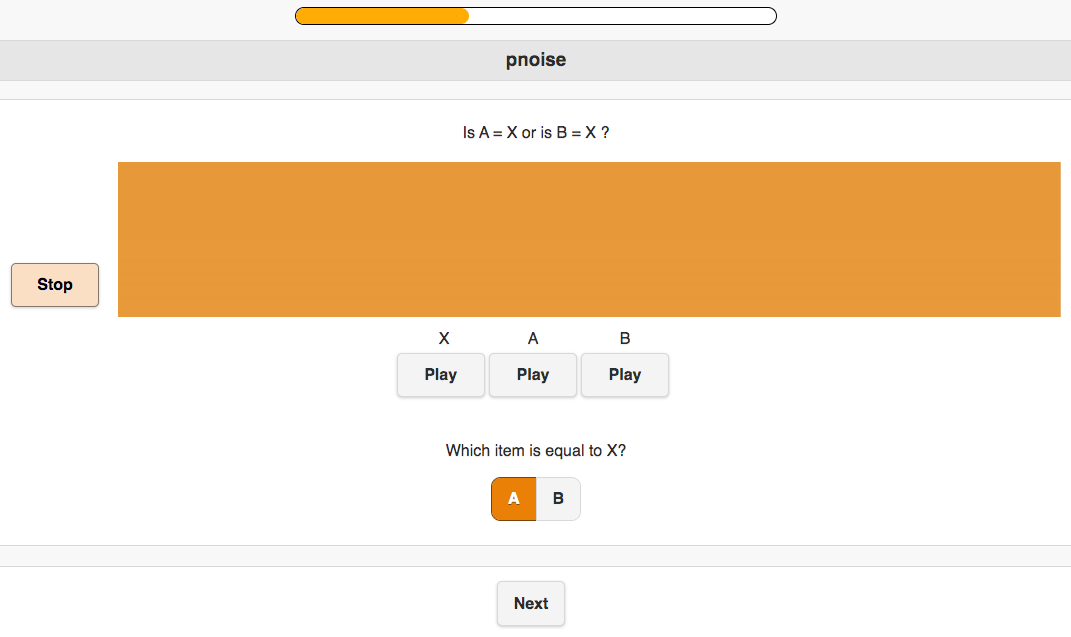
\includegraphics[width=\textwidth]{graphics/abx_gui}};
\node at (9.5,-1.4)
{
\begin{tabular}{ |c|c|c| }
 \hline
 X & A & B \\\hline
 original & phase & original \\
 phase & phase & original \\
 original & original & phase \\
 phase & original & phase \\
 \hline
\end{tabular}
};
\node at (3,-4){\tiny\url{https://www.audiolabs-erlangen.de/resources/webMUSHRA}};
\end{tikzpicture}
\end{frame}
%
%
%
\begin{frame}{Audio Material Considerations}
\begin{tikzpicture}[remember picture,overlay]
\node at (9,-5) {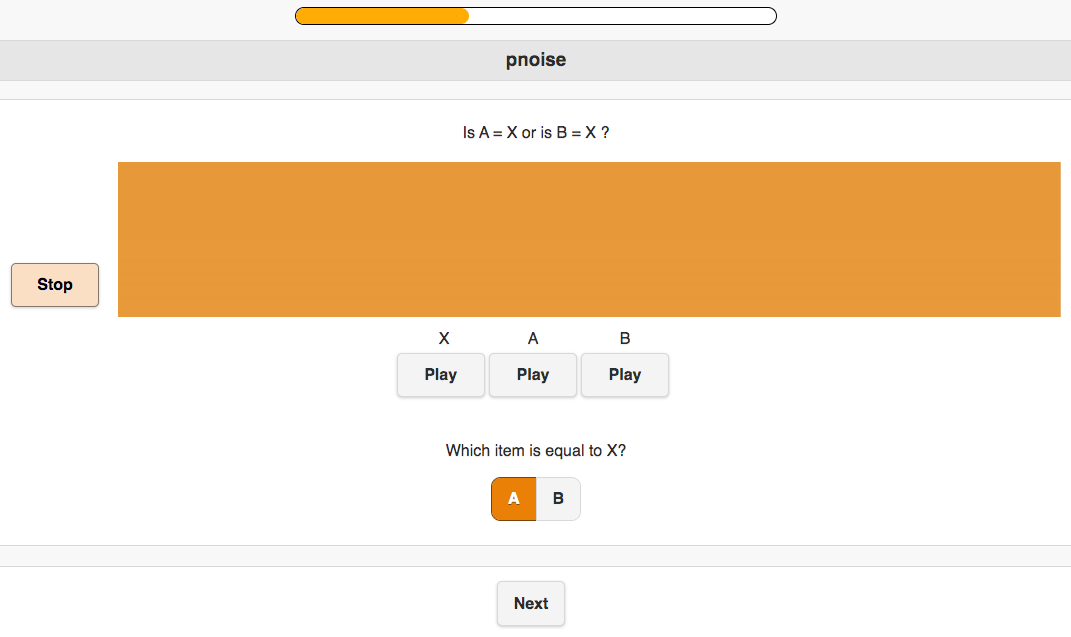
\includegraphics[width=0.5\textwidth]{graphics/abx_gui}};
\end{tikzpicture}
%
\textbf{4x Audio}
\begin{itemize}
\item square wave bursts 50 Hz, 200 ms on, 300ms off, $\sin^2$ fades
\item 300Hz-lowpass filtered pink noise
\item castanets (anechoic by Matthias Frank)
\item music excerpt with percussion, drums (Eagles, Hotel California, Hell freezes over, 1994)
\end{itemize}
%
\vspace*{0.25cm}
%
\textbf{5x Treatment}: Constant Phase Shift vs. Original ($\varphi = 0\degree$)
\begin{enumerate}[I]
\item square wave bursts with $\mathcolor{colnonzero}{\varphi=-90\degree}$
\item square wave bursts with $\mathcolor{colzerotalk}{\varphi=-45\degree}$
\item lowpass filtered pink noise with $\mathcolor{colnonzero}{\varphi=-90\degree}$
\item castanets with $\mathcolor{colnonzero}{\varphi=-90\degree}$
\item Hotel California with $\mathcolor{colnonzero}{\varphi=-90\degree}$
\end{enumerate}
\end{frame}
%
%
%
\begin{frame}{ABX Test Statistic Considerations}
\textbf{Sloppy} formulation of our research question:

Is the number of correct answers (either A=X or B=X was correctly discriminated)
higher than pure guessing would indicate?
\vspace{0.25cm}

\textbf{PreHoc}:
\begin{itemize}
\item
null hypothesis $\Hnull(p_\text{detect}=0.5)$
\item
subjects are to rate 5 treatments $\rightarrow$ Bonferroni correction for individual $\alpha_\text{I...V}, \beta_\text{I...V}$
\item
target rejection level $\alpha=0.05$
\item
target test power $1-\beta = 0.95$

\item
assumed effect size $g=0.4$ due to estimated $p_\text{detect}=0.9$ in preliminary tests
\item
\textcolor{colnonzero}{per audio content}:
for $\frac{\geq 19\,\text{correct trials}}{25\,\text{total trials}}
\rightarrow p_\text{Binomial PDF}<\frac{\alpha}{5} \rightarrow\Hnull$
can be rejected
\end{itemize}
%
\vspace{0.25cm}

\textbf{PostHoc}:

pairwise comparisons w.r.t. detection frequencies for small/medium effect size
with $\chi^2$-distribution/-test

\end{frame}
%
%
%
\begin{frame}{Listening Experiment Conditions}
\begin{itemize}
\item participants: 4 female, 8 male
\item ratings: 12 participants x 5 treatments x 25 trials per treatment
\item fully randomized stimuli sequence
\item loudspeaker lab, 40 dB(A) noise floor, mean RT 0.3s
\item diotic playback via \textcolor{colzerotalk}{headphone} Sennheiser HD800
\item all stimuli loudness matched according to ITU-R BS.1770-4, except castanets
\item $72.7~\text{dB(A)}_\text{Leq}$ / $87.7~\text{dB(C)}_\text{Peak}$
for fullband pink noise
\end{itemize}
\begin{figure}
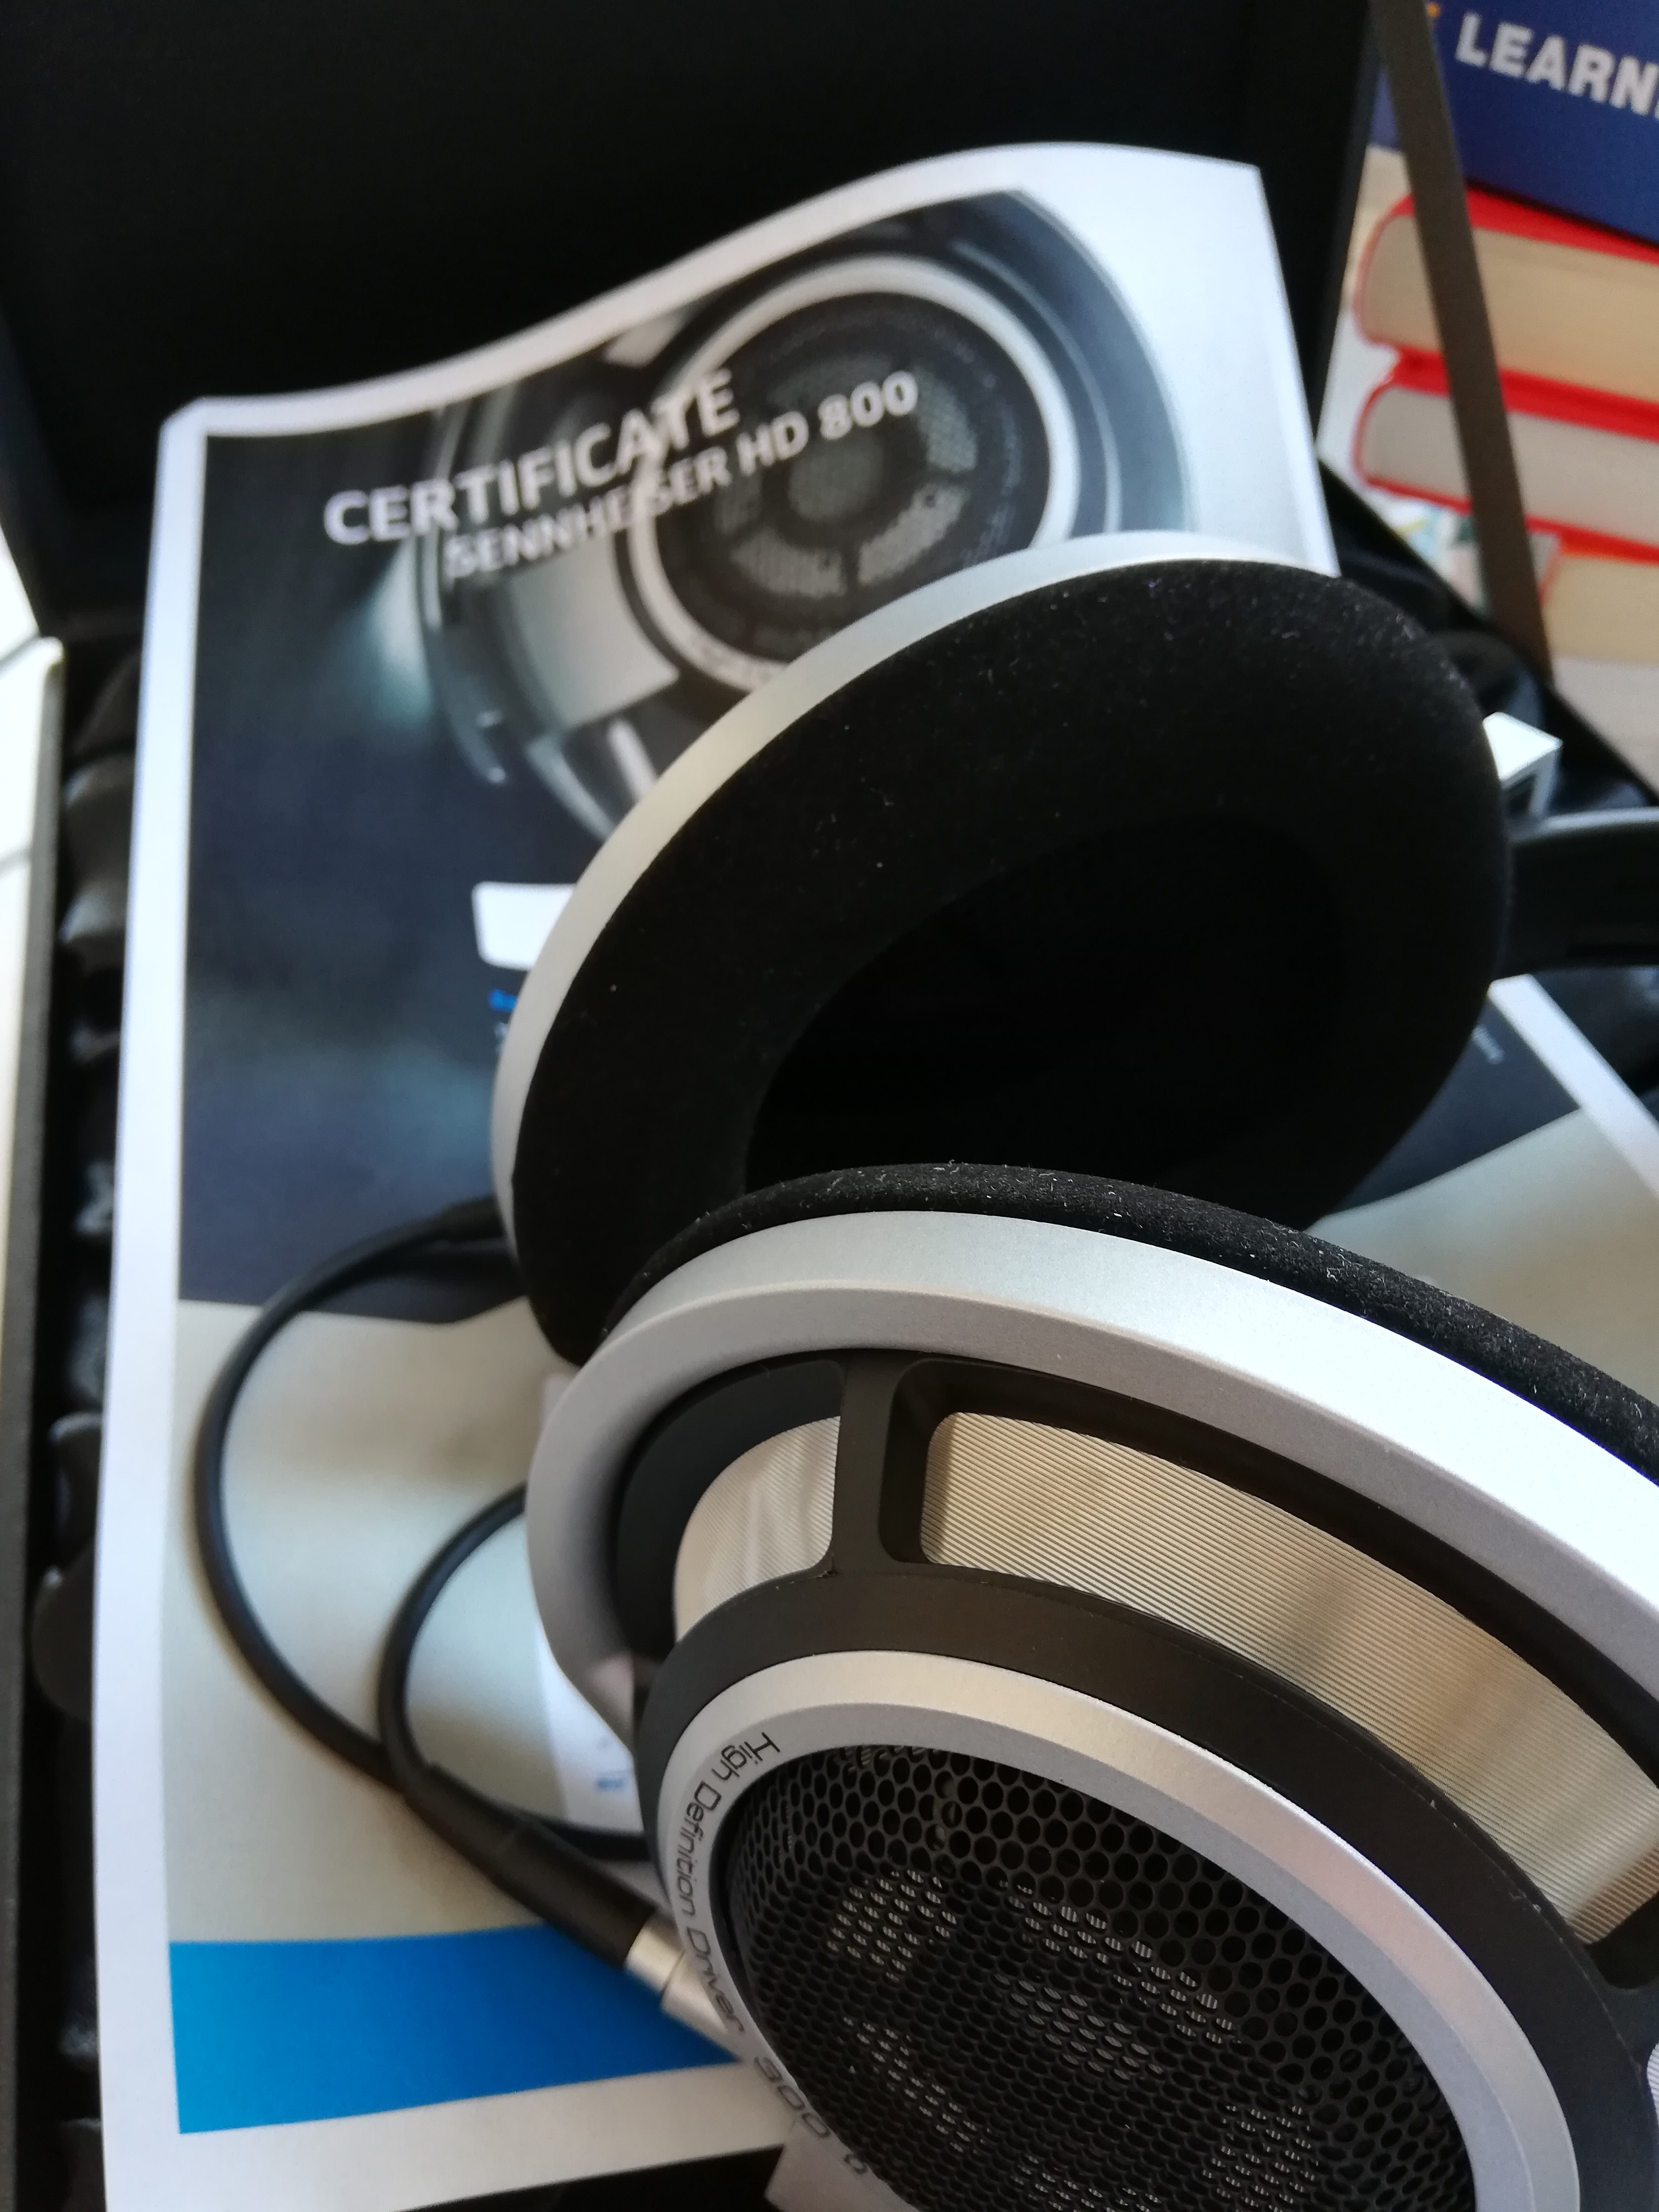
\includegraphics[width=0.25\textwidth]{graphics/HD800}
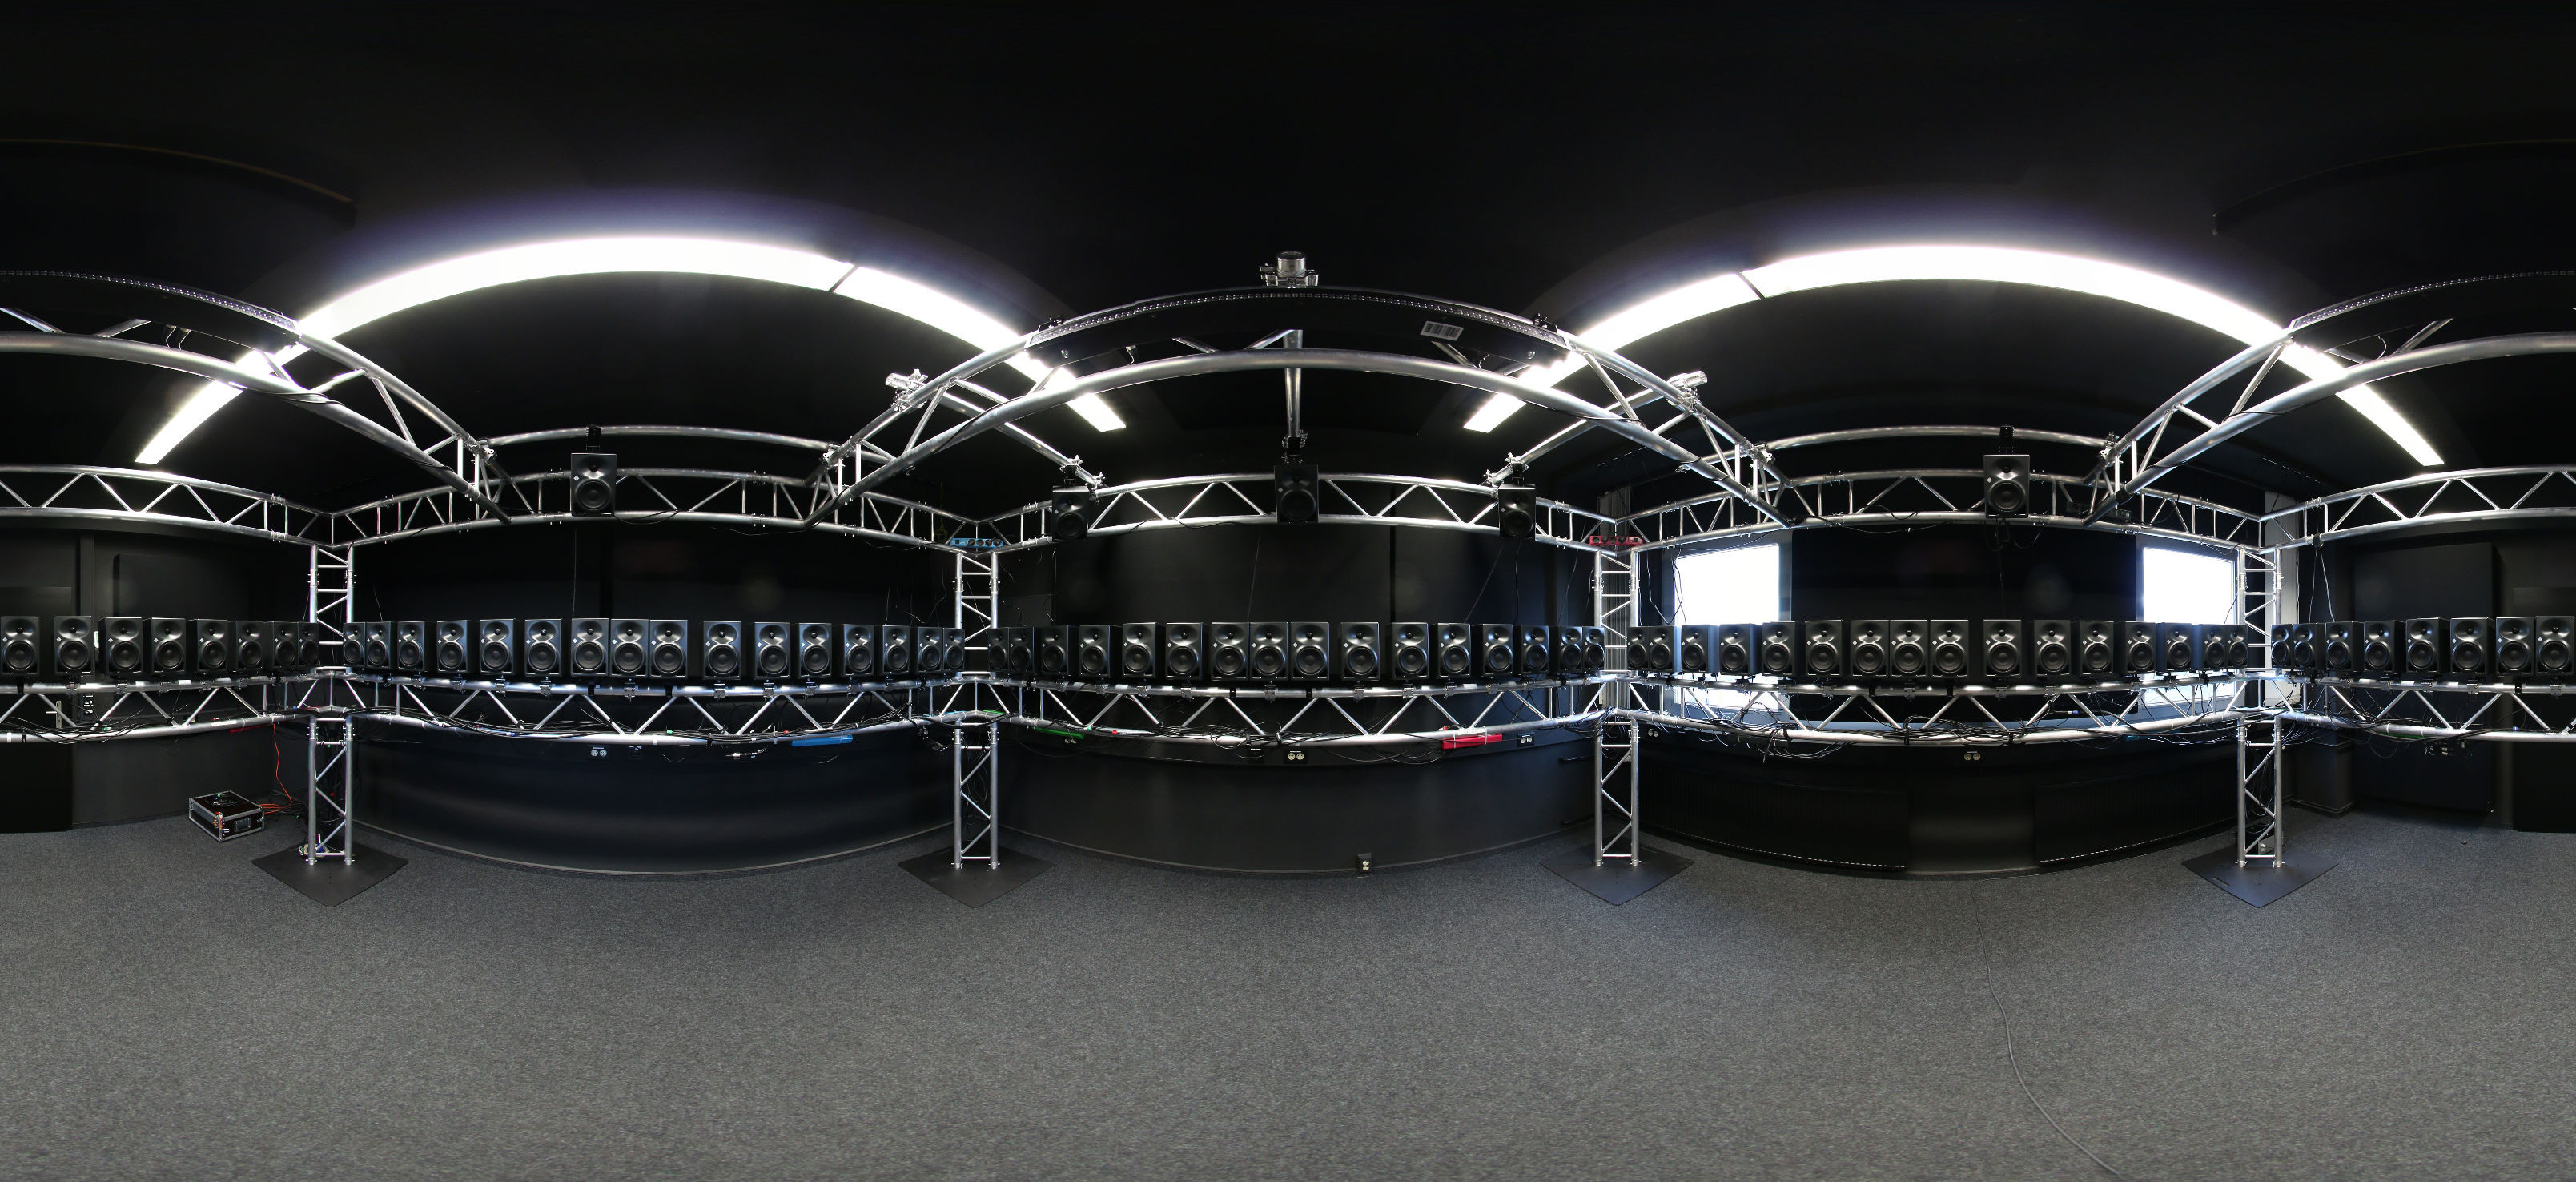
\includegraphics[width=0.6\textwidth]{graphics/URO_array_panorama}
\end{figure}

\end{frame}
%
%
%
\begin{frame}{Listening Experiment Results}
\begin{figure}
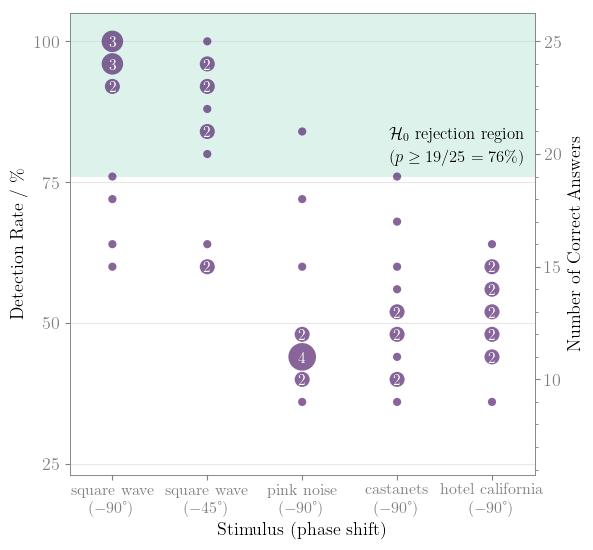
\includegraphics[width=0.75\textwidth]{graphics/scatter}
\end{figure}
\end{frame}
%
%
%
\section{Conclusion}
\begin{frame}{Conclusion}
constant phase shifter is known as fractional Hilbert transform

audibility depends on audio material and amount of constant phase shift

\begin{columns}[c]
\column{0.45\textwidth}
\begin{figure}
\includegraphics[width=1\textwidth]{graphics/spectra_filterorder510}
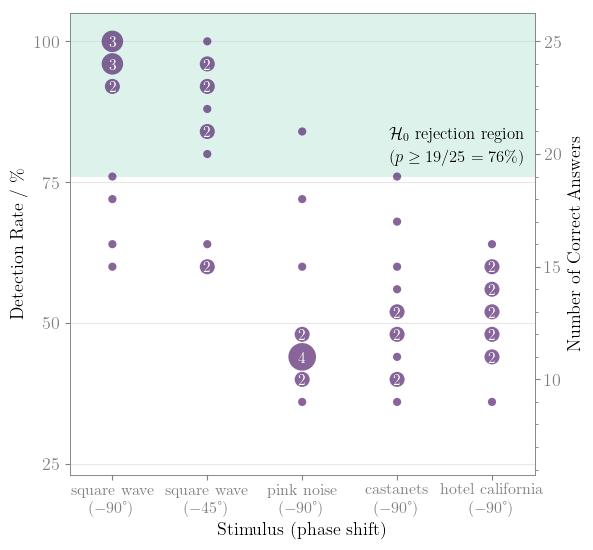
\includegraphics[width=1\textwidth]{graphics/scatter}
\end{figure}
\column{0.5\textwidth}
\only<1>{
\begin{itemize}
\item very sensitive to square wave bursts
\item likely sensitive for transient signals and lowpass filtered noise
\item audibility for musical content not yet shown
\item training improves sensitivity...
\end{itemize}
}
\only<2>{

\textcolor{colnonzero}{\textbf{Outlook}}

trained experts achieve

%\textcolor{colnonzero}{pink noise}: 40 correct detections $(p<2.1 \cdot 10^{-10})$
%\textcolor{colnonzero}{castanets}: 28 correct $(p<0.022)$ and 39 correct $(p<2.9\cdot10^{-9})$

\textcolor{colnonzero}{pink noise} $\mathcolor{colnonzero}{\varphi=-90\degree}$:

95\% correct answers $(p<2.1 \cdot 10^{-10})$

\textcolor{colnonzero}{castanets} $\mathcolor{colnonzero}{\varphi=-90\degree}$:

92\% correct answers $(p<2.9\cdot10^{-9})$
\vspace*{0.5cm}

\tiny ABX test design with assumed effect size $g =	0.25$,
$\alpha = 0.05$, power $1-\beta=0.95 \rightarrow
\frac{\geq 27\,\text{correct trials}}{42\,\text{total trials}}$
}
\end{columns}
\end{frame}
%
%
%
\author{%
    Frank Schultz,
    Nara Hahn,
    Sascha Spors
}
\institute{University of Rostock}
\date{Open Science: https://doi.org/10.5281/zenodo.\textcolor{colzerotalk}{3383286}}
\maketitle
%
%
%
\section{Appendix}
%
%
%
\begin{frame}[noframenumbering]{Periodic Convolution}
Impulse response for $\varphi=-\frac{\pi}{4}$
\begin{figure}
\includegraphics[width=0.75\textwidth]{graphics/periodic-ir}
\end{figure}
\end{frame}
%
%
%
\begin{frame}[noframenumbering]{Quantization Filter Coefficients}
\begin{figure}
\includegraphics[width=\textwidth]{graphics/amplitude-decay}
\end{figure}
\end{frame}
%
%
%
\begin{frame}[noframenumbering]{Crest Factor}
\begin{figure}
\includegraphics[width=\textwidth]{graphics/crest-factor-and-square-waves}
\end{figure}
\end{frame}
%
%
%
\begin{frame}[noframenumbering]{Crest Factor}
\begin{figure}
\includegraphics[width=\textwidth]{graphics/crest-factor}
\end{figure}
\end{frame}
%
%
%
\end{document}
